\documentclass[border=3pt]{standalone}
\usepackage[T1]{fontenc}
\usepackage{helvet}
\renewcommand{\familydefault}{\sfdefault}
\usepackage{tikz}
\usetikzlibrary{arrows.meta,positioning,fit,backgrounds,shapes.geometric,calc}
\definecolor{ink}{HTML}{1F3A56}
\definecolor{core}{HTML}{DCE7F2}
\definecolor{know}{HTML}{DDEFE8}
\definecolor{game}{HTML}{F6E8D6}
\definecolor{model}{HTML}{EAE3F3}
\definecolor{plain}{HTML}{F3F4F6}
\definecolor{bad}{HTML}{B3402E}
\tikzset{
 every node/.style={font=\fontsize{8.5}{10.2}\selectfont,align=center,text=ink,execute at begin node={\hyphenpenalty=10000\exhyphenpenalty=10000}},
 box/.style={draw=ink,fill=white,rounded corners=1.5pt,minimum height=8.5mm,inner sep=3pt,line width=.5pt},
 corebox/.style={box,fill=core},
 knowbox/.style={box,fill=know},
 gamebox/.style={box,fill=game},
 modelbox/.style={box,fill=model},
 plainbox/.style={box,fill=plain},
 planned/.style={dashed},
 flow/.style={-{Stealth[length=2mm]},draw=ink,line width=.6pt},
 dflow/.style={flow,dashed},
 badflow/.style={flow,draw=bad,dashed},
 band/.style={draw=ink!55,rounded corners=3pt,inner sep=6pt,line width=.45pt},
 title/.style={font=\bfseries\fontsize{8.5}{10.2}\selectfont},
 lab/.style={font=\fontsize{7.5}{9}\selectfont,fill=white,inner sep=1pt},
 decision/.style={diamond,draw=ink,fill=core,aspect=2.1,inner sep=0.5pt,line width=.5pt}
}

\begin{document}
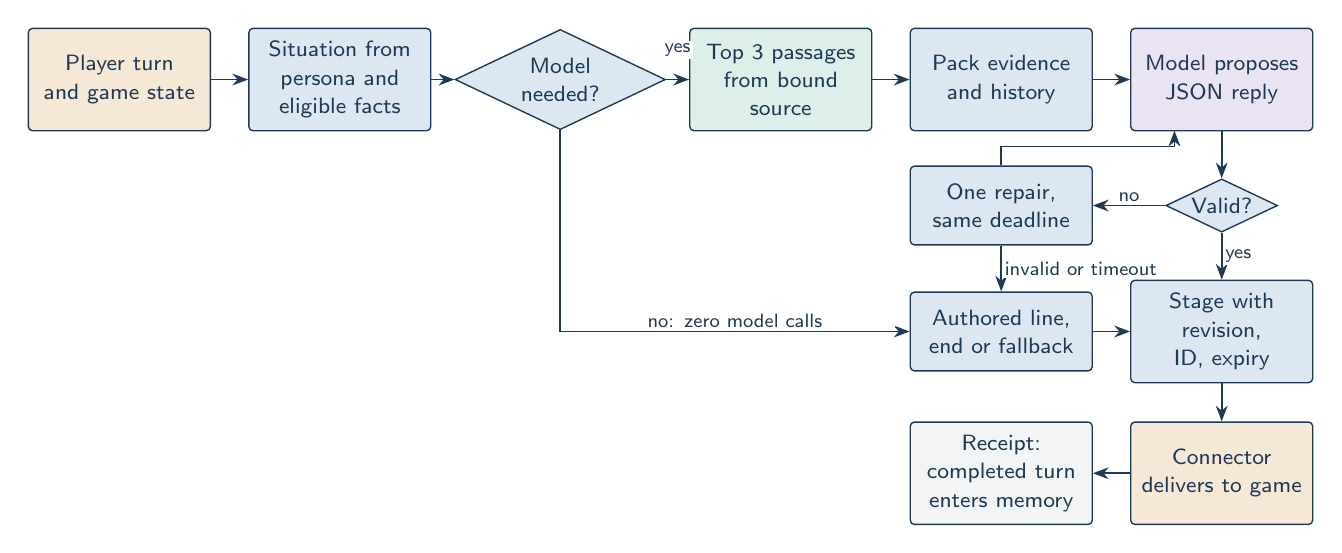
\begin{tikzpicture}[x=1mm,y=1mm]
\def\tw{21mm}
% Column centres 12, 40, 68, 96, 124, 152
\node[gamebox,text width=\tw,minimum height=13mm] (in) at (12,40) {Player turn and game state};
\node[corebox,text width=\tw,minimum height=13mm] (ctx) at (40,40) {Situation from persona and eligible facts};
\node[decision,text width=14mm] (route) at (68,40) {Model needed?};
\node[knowbox,text width=\tw,minimum height=13mm] (rag) at (96,40) {Top 3 passages from bound source};
\node[corebox,text width=\tw,minimum height=13mm] (prompt) at (124,40) {Pack evidence and history};
\node[modelbox,text width=\tw,minimum height=13mm] (llm) at (152,40) {Model proposes JSON reply};
\node[decision,text width=9mm] (ok) at (152,24) {Valid?};
\node[corebox,text width=\tw,minimum height=10mm] (repair) at (124,24) {One repair, same deadline};
\node[corebox,text width=\tw,minimum height=10mm] (auth) at (124,8) {Authored line, end or fallback};
\node[corebox,text width=\tw,minimum height=13mm] (stage) at (152,8) {Stage with revision, ID, expiry};
\node[gamebox,text width=\tw,minimum height=13mm] (deliver) at (152,-10) {Connector delivers to game};
\node[plainbox,text width=\tw,minimum height=13mm] (mem) at (124,-10) {Receipt: completed turn enters memory};
\draw[flow] (in) -- (ctx);
\draw[flow] (ctx) -- (route);
\draw[flow] (route) -- node[lab,above,yshift=2.5mm] {yes} (rag);
\draw[flow] (rag) -- (prompt);
\draw[flow] (prompt) -- (llm);
\draw[flow] (llm) -- (ok);
\draw[flow] (ok) -- node[lab,above] {no} (repair);
\draw[flow] (repair.north) |- (146,31.5) -- (146,33.5);
\draw[flow] (ok) -- node[lab,right] {yes} (stage);
\draw[flow] (repair) -- node[lab,right] {invalid or timeout} (auth);
\draw[flow] (route.south) |- node[lab,pos=.75,above,text width=40mm] {no: zero model calls} (auth.west);
\draw[flow] (auth) -- (stage);
\draw[flow] (stage) -- (deliver);
\draw[flow] (deliver) -- (mem);
\end{tikzpicture}
\end{document}
